\documentclass{article}
\usepackage{arxiv}
\usepackage{wrapfig}
\usepackage{amsmath}
\usepackage[utf8]{inputenc}
\usepackage[english]{babel}
\usepackage[T1]{fontenc}
\usepackage{url}
\usepackage{booktabs}
\usepackage{float}
\usepackage{amsfonts}
\usepackage{diagbox}
\usepackage{nicefrac}
\usepackage{microtype}
\usepackage{lipsum}
\usepackage{amssymb}
\usepackage{graphicx}
\usepackage{natbib}
\usepackage{doi}
\usepackage{makecell}
\usepackage{subfig}

\pagestyle{fancy}

\title{Calculating the value of a multivariate time series at a point by the predicted matrix of pairwise correlation}

\author{ Maxim Divilkovskiy \\
% \thanks{Use footnote for providing further
% 		information about author (webpage, alternative
% 		address)---\emph{not} for acknowledging funding agencies.} \\
	Chair of Data Analysis\\
	MIPT\\
	\texttt{divilkovskii.mm@phystech.edu} \\
	%% examples of more authors
	\And Gleb Karpeev \\
	% \thanks{Use footnote for providing further
		% 		information about author (webpage, alternative
		% 		address)---\emph{not} for acknowledging funding agencies.} \\
	MIPT\\
	\texttt{karpeev.ga@phystech.edu} \\
	%% examples of more authors
	\And
	Vadim Strijov \\
	FRC CSC of the RAS\\
	Moscow, Russia\\
    \texttt{strijov@phystech.edu} \\
    \And
    Konstantin Yakovlev \\
    Chair of Intellectual Systems\\
    MIPT\\
    \texttt{iakovlev.kd@phystech.edu} \\
	% Santa Narimana, Levand \\
	% \texttt{stariate@ee.mount-sheikh.edu} \\
	%% \AND
	%% Coauthor \\
	%% Affiliation \\
	%% Address \\
	%% \texttt{email} \\
	%% \And
	%% Coauthor \\
	%% Affiliation \\
	%% Address \\
	%% \texttt{email} \\
	%% \And
	%% Coauthor \\
	%% Affiliation \\
	%% Address \\
	%% \texttt{email} \\
}
\date{}

\renewcommand{\shorttitle}{\textit{arXiv} Template}

%%% Add PDF metadata to help others organize their library
%%% Once the PDF is generated, you can check the metadata with
%%% $ pdfinfo template.pdf
\hypersetup{
pdfauthor={Maxim Divilkovskiy},
}

\graphicspath{ {./figures/} }

\begin{document}
\maketitle

\begin{abstract}
	We are researching the problem of pointwise forecasting of a set of time series with high covariance and high variance. To solve this problem we propose considering the space of pairwise distances between time series. In this space the pairwise distance matrix is predicted and then the time series values at the next time moment are reconstructed using the known matrix. In this paper we propose several methods for recovering a prediction in time series space from a known pairwise distance matrix. We show the existence of multiple time series values satisfying the same pairwise distance matrix. We propose two algorithms based on the use of matrices constructed over different time intervals using pairwise correlation. Also, the paper derives an explicit view of the recovered values through the pairwise correlation matrix. In addition, we derive an evaluation of the quality of the reconstruction when noise is added to the pairwise distance matrices. The novelty of the method is that the prediction is not done in the original space, but in the space of pairwise distances.


\end{abstract}


\keywords{Metric \and Non-Convex Optimization \and Singular Value Decomposition \and Pearson Correlation Coefficient \and Time Series Forecasting}

\section{Introduction}
 	In this research we present a new method for pointwise time series forecasting. Considered time series are characterized by high pairwise covariance and high variance. The task of pointwise forecasting is to calculate the values of time series at the next point in time using the available historical data for the previous several points in time. The task is divided into three stages: first, the initial space of time series is transformed into a metric space by constructing a matrix of pairwise distances. Then the prediction of the matrix of pairwise distances at the next moment of time is done in the metric space. In the theoretical part of the paper, we show the necessity of predicting at least two matrices. We also show that the uniqueness of the answer requires the use of several matrices corresponding to different time intervals. In the last step, the predicted matrices are used to reconstruct the result into the original space. We focus mostly on the last step. Experiments are presented for the case of accurate matrix prediction with the addition of normal noise to the values.

	Existing time series prediction methods such as LSTM \cite{LSTM}, SSA \cite{SSA} and other \cite{Biosignals}, \cite{boyd2017multiperiod} are based on predicting the value of a single series. These methods can be modified to forecast also a set of time series. For this purpose, it is sufficient to consider a set of series as one multivariate series. However, this approach does not explicitly model the dependencies between different series. In this paper, we propose to analyze the change in \textit{set} of time series. This approach explicitly uses the relationships between them as information. A similar study is carried out in the \cite{MulticorrelatedQuadratic} paper, but it emphasizes on the feature selection task. This task consists in selecting such a subset of the original time series for which it is possible to make a forecast of sufficient quality.
	
	Several recent studies \cite{haoyietal-informer-2021} \cite{haoyietal-informerEx-2023} \cite{wu2021autoformer} \cite{liu2022pyraformer} are based on usage of popular transformer-based models. They were originally proposed for the natural language processing problems, such as translation and text-completion \cite{NIPS2017_3f5ee243}. However, since many language problems dealing with text as a sequence in time, same approaches may be used for time series predicting. Crossformer \cite{zhang2023crossformer} model uses cross-dimensional dependency, however it does not explicitly model distance function between time series.
	
	Further, we study conditions on the distance function between rows under which there is a way to recover the values of time series. The insufficiency of one matrix to recover the answer is proved. Two methods using several matrices are proposed for the case of accurate forecast and for the case of forecast with non-zero noise. Also, we propose a reconstruction algorithm based on two theorems about the explicit formula of the result in time series space using pairwise correlation as a function of pairwise distance between rows. Mean Squared Error and Mean Absolute Error are used as quality criteria. It is shown in the article \cite{jadon2022comprehensive} that they are the most suitable for the task of time series forecasting.

\section{Formulation of the problem of pointwise forecasting of a set of time series}

A set of $d$ time series is given by $t$ vectors:

$$[\mathbf{x}_1, \mathbf{x}_2, \ldots, \mathbf{x}_t], \text{for each } k: \mathbf{x}_k \in \mathbb{R}^d, $$

$\mathbf{x}_{t_i, k} \in \mathbb{R}$ is the value of the series with index $k$ at the time moment $t_i$.

The task is to predict $\mathbf{x}_{t+1}$~--- the set of values of all time series at the time moment $t+1$.

The matrix $\mathbf{x}$ of size $t \times d$ is treated as a \textit{multidimensional} time series, treating the value at a point as an element of space $\mathbb{R}^d$.

Prediction errors are calculated using the following equations:
\[
\text{MAE} = \frac{\sum_{i=1}^{d} |\mathbf{x_{t+1}} - \mathbf{\hat{x}_{t+1}}|}{d},
\]

\[
\text{MSE} = \frac{\sum_{i=1}^{d} (\mathbf{x_{t+1}} - \mathbf{\hat{x}_{t+1}})^2}{d}.
\]

\section{Algorithm in case of predicting a single distance matrix}

1. Distance matrices between a set of time series values are constructed according to the scheme below.
\begin{align*}
	[\mathbf{x}_1, \ldots, \mathbf{x}_s] &\rightarrow \mathbf{\Sigma}_s, \\
	[\mathbf{x}_2, \ldots, \mathbf{x}_{s+1}] &\rightarrow \mathbf{\Sigma}_{s+1}, \\
	&\vdots \\
	[\mathbf{x}_{t-s}, \ldots, \mathbf{x}_t] &\rightarrow \mathbf{\Sigma}_{t}.
\end{align*}

Each $\mathbf{\Sigma}_i$~--- is a matrix of pairwise distances of size $d \times d$. An element of the matrix $\mathbf{\Sigma}_{i,j}$ is the value of the distance between rows $i$ and $j$. The construction formula as well as the choice of the distance function are described in the following sections.

2. The matrix $\hat{\mathbf{\Sigma}}_{t+1}$ is predicted from these matrices.

3. Find such $\mathbf{\hat{x}}_{t+1}$, that \[ ||\hat{\mathbf{\Sigma}}_{t+1} - \bar{\mathbf{\Sigma}}_{t+1}||_2^2 \] is minimal, where $\bar{\mathbf{\Sigma}}_{t+1}$ is the distance matrix, constructed from the set $[\mathbf{x}_{t-s+1}, \ldots, \mathbf{x}_{t}, \mathbf{\hat{x}}_{t+1}]$. Achieving a minimum by this function would mean that $\hat{\mathbf{\Sigma}}_{t+1}$ are $\bar{\mathbf{\Sigma}}_{t+1}$ equal. In turn, this means that the found continuation of the series at time $t+1$ has a distance matrix equal to the prediction. In general, this function is \textit{non-convex} and there can be several minimums. We address this problem in the following sections.

\section{Existence of several values of a series satisfying same distance matrix}

The existence of several solutions to the minimization problem described above is the central problem we consider in this paper. In this section we show that using one matrix constructed by an arbitrary metric it is possible to recover several different values of the series at the next moment of time. A solution to this problem in the case of using pairwise correlation as a function of distance between certain time series is proposed in the next section.

Consider the reconstruction of the prediction from the matrix $\mathbf{\Sigma}_{t+1}$ to time series space, where $\mathbf{\Sigma}_{t+1}$ is the matrix of pairwise distances corresponding to the multivariate series $\mathbf{x}=[\mathbf{x_1}, \ldots, \mathbf{x_{t+1}}]$.

Given a pairwise distance matrix $\mathbf{\Sigma}$ of size $d \times d$ for multivariate time series $\mathbf{x} \in \mathbb{R}^{d \times (t+1)}$. $\hat{\mathbf{x}}_{t+1} \in \mathbb{R}^d$ is predicted. Also, the metric \[ \rho : \mathbb{R}^{t+1} \times \mathbb{R}^{t+1} \rightarrow \mathbb{R}, \] defined on time series, which satisfies the properties of the metric. Which are \[\mathbf{\Sigma}_{i,j} = \rho(\mathbf{x}_{1 \ldots t, i} \circ \hat{\mathbf{x}}_{t+1, i}, \mathbf{x}_{1 \ldots t, j} \circ \hat{\mathbf{x}}_{t+1, j}),\] where $\circ$ denotes the concatenation of vector with value.

One of the fundamentally metrics for calculating distance of objects in $\mathbb{R^d}$ is the Euclidean metric. On this example, we will show that there can be several suitable answers with the same values of distance matrix. Moreover, in the case of the Euclidean metric, the number of answers is infinite, which is shown below:
\[\mathbf{\Sigma}_{i,j} = \rho(\mathbf{x}_{1 \ldots t, i} \circ \hat{\mathbf{x}}_{t+1, i}, \mathbf{x}_{1 \ldots t, j} \circ \hat{\mathbf{x}}_{t+1, j})=\sqrt{\left(\sum_{k=1}^t (\mathbf{x}_{k,i}-\mathbf{x}_{k,j})^2\right) + (\hat{\mathbf{x}}_{t+1, i}-\hat{\mathbf{x}}_{t+1, j})^2}.\]

Using this metric results in the fact that adding some constant $C$ to all $\hat{\mathbf{x}}_{t+1, i}$ does not change the answer:
\[
\sqrt{\left(\sum_{k=1}^t (\mathbf{x}_{k,i}-\mathbf{x}_{k,j})^2\right) + (\hat{\mathbf{x}}_{t+1, i}-\hat{\mathbf{x}}_{t+1, j})^2} = \sqrt{\left(\sum_{k=1}^t (\mathbf{x}_{k,i}-\mathbf{x}_{k,j})^2\right) + [(\hat{\mathbf{x}}_{t+1, i} + C) -(\hat{\mathbf{x}}_{t+1, j} + C)]^2}.
\]

In the case of the time series prediction problem, this property is critical because even if the matrix $\mathbf{\Sigma}$ is predicted accurately, there are infinitely many time series values at time $t+1$ corresponding to this matrix. See \ref{fig:fig1} for the example of this effect.
\begin{figure}[H]
	\centering
	\subfloat[Reference functions]{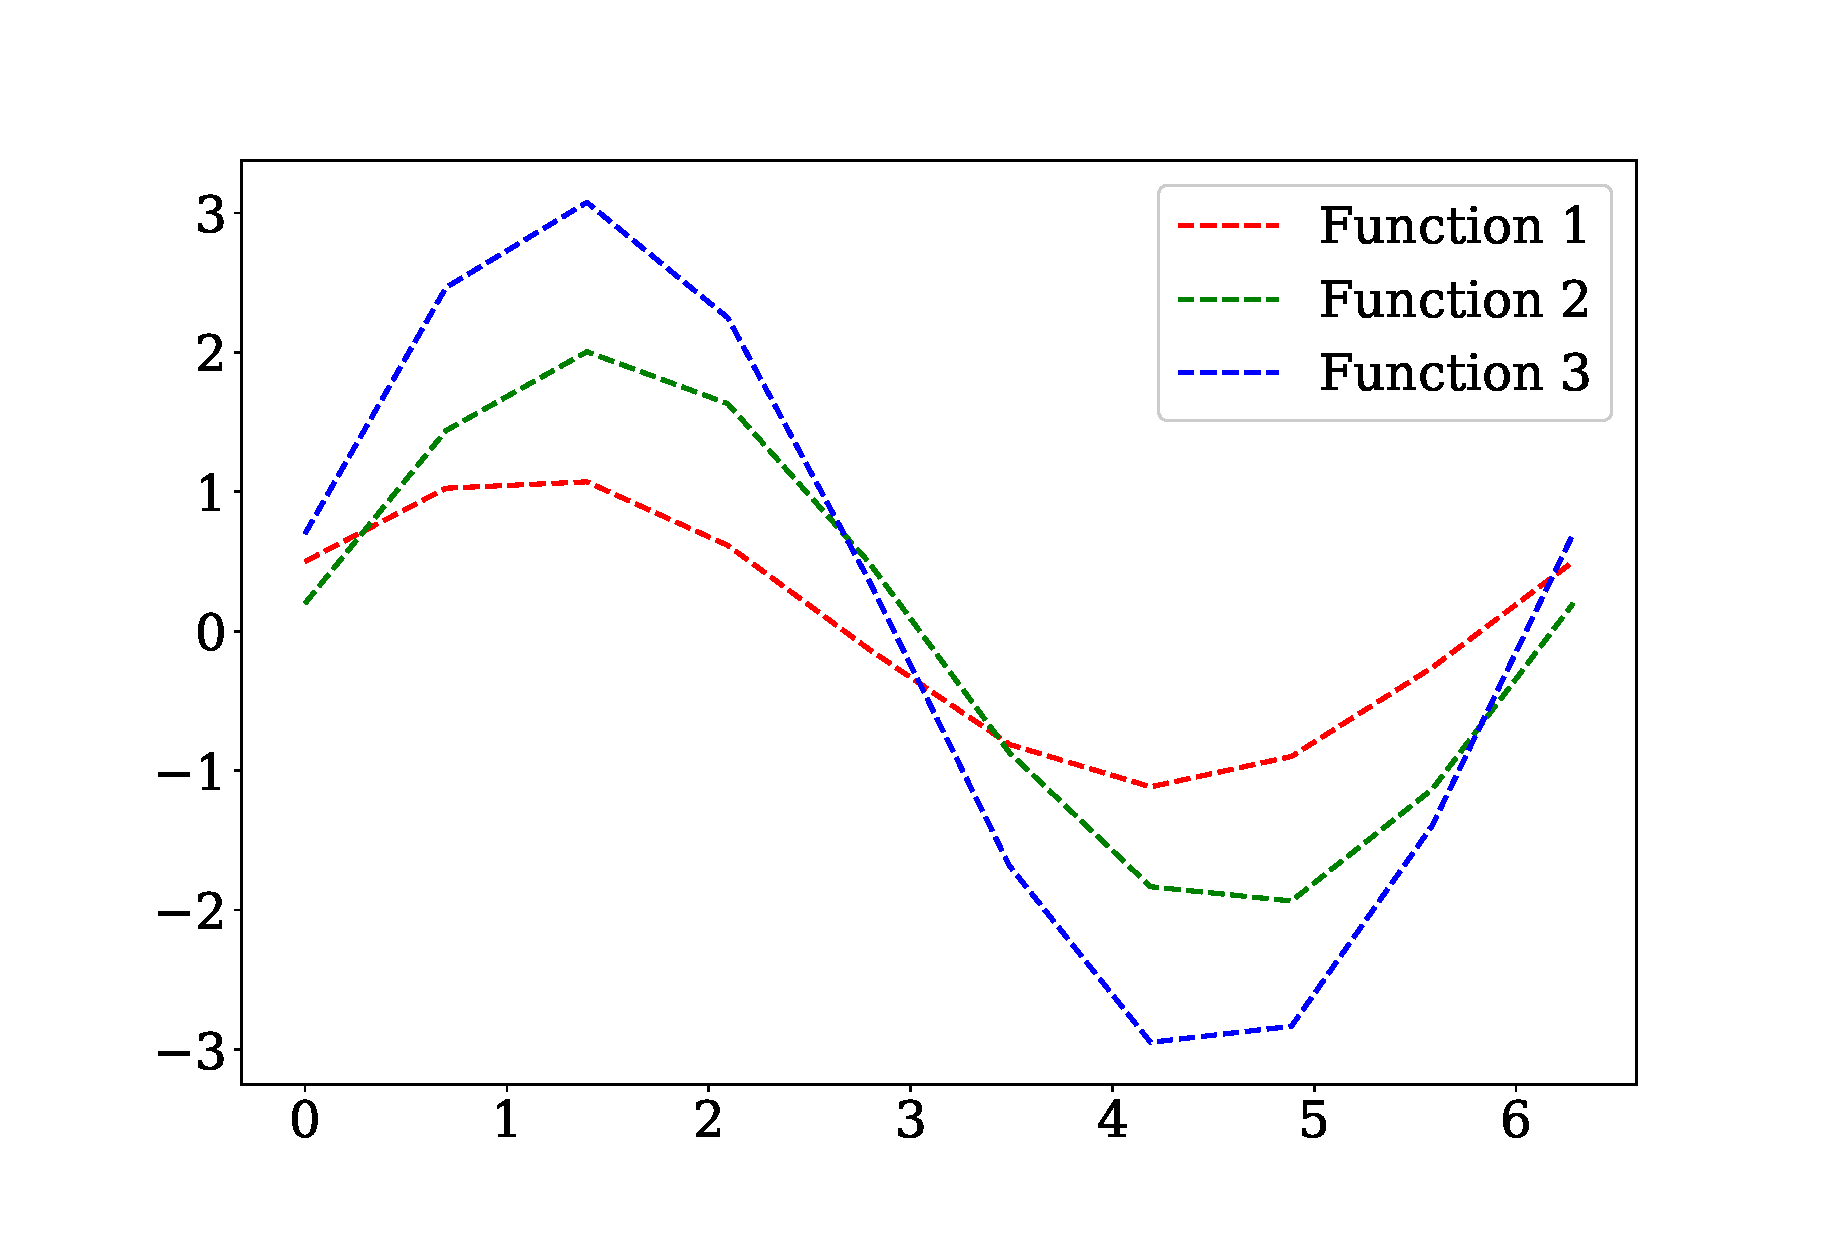
\includegraphics[width=0.5\textwidth]{Original_functions.eps}}
	\subfloat[Modified functions where 3 is subtracted from the last values]{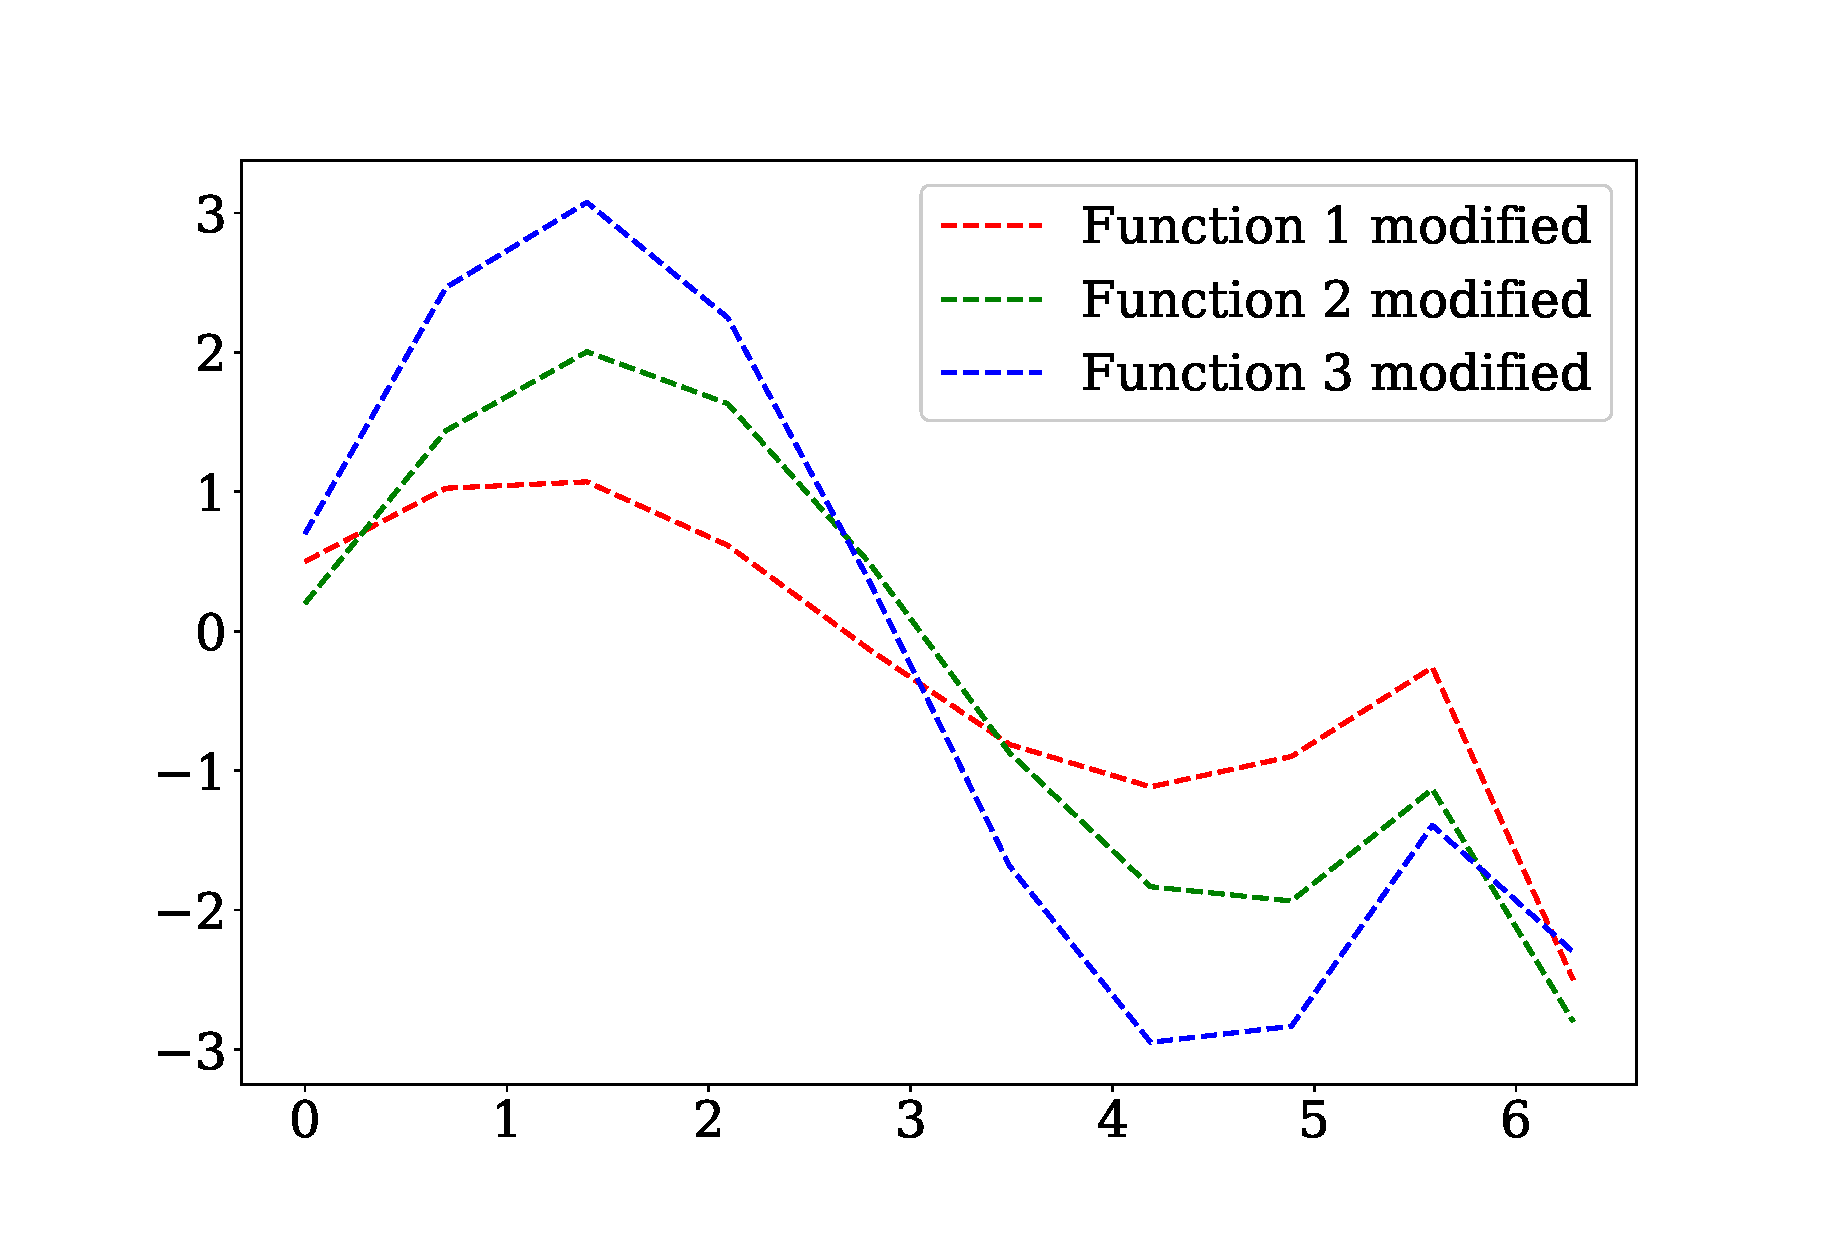
\includegraphics[width=0.5\textwidth]{Modified_functions.eps}}\\
	\caption{These sets of time series have the same distance matrix constructed on the Euclidean metric.}
	\label{fig:fig1}
\end{figure}

However, even using other metrics does not get rid of the problem. This results in the inability to use the classical Multidimentional Scaling \cite{MDS} algorithm to recover the response to the source time series space. This algorithm is often used to recover objects from their pairwise distances. Metric MDS Algorithm  \cite{inbook} may be used if distances are not euclidean.

In the theorem below we show that usage of only one matrix is insufficient for the problem of recovering values of time series.

\textbf{Theorem 1.} \textit{For any metric $\rho$ defined in the time series space $\mathbb{R}^t$ there is more than one way to recover the original time series from the pairwise distance matrix constructed by the given metric.}	

\textbf{Note 1}. This statement does not use information about the first $t-1$ values of the series. In fact, the series in this case can be thought of as a point in $\mathbb{R}^t$ space. The usage of information about the previous moments of time is considered after this section.

\textbf{Proof}. We only have to show that the metric is not a bijection. This will mean that there are several different pairs of series whose distance between them is the same.

Let us show that the metric is a continuous function. Take the sequence \[\{(\mathbf{x}_n, \mathbf{y}_n)\} \subset \mathbb{R}^t \times \mathbb{R}^t, (\mathbf{x}_n, \mathbf{y}_n) \to (\mathbf{x}, \mathbf{y}).\] Then, \[\mathbf{x}_n\to \mathbf{x}, \mathbf{y}_n\to \mathbf{y} \Rightarrow \rho(\mathbf{x}_n,\mathbf{x})\to 0 ,\rho(\mathbf{y}_n,\mathbf{y})\to 0,\] $n \to \infty.$ Using the triangle inequality for the metric, we obtain \[\rho(\mathbf{x}_n,\mathbf{y}_n)\leqslant \rho(\mathbf{x}_n,\mathbf{x})+\rho(\mathbf{x},\mathbf{y})+\rho(\mathbf{y}_n,\mathbf{y})\to \rho(\mathbf{x},\mathbf{y}),\] therefore, $\rho(\mathbf{x}_n,\mathbf{y}_n)\to \rho(\mathbf{x},\mathbf{y})$.

Therefore the metric is a continuous mapping from $\mathbb{R}^t \times \mathbb{R}^t$ to $\mathbb{R}$. We will show that such a mapping cannot be a homeomorphism. Assume that $f: \mathbb{R} \to \mathbb{R}^t \times \mathbb{R}^t$ is the desired homeomorphism. Take arbitrary point $a \in \mathbb{R}$ and $f(a)$. Removing point $a$, $\mathbb{R}$ is no longer connected, but $\mathbb{R}^t \times \mathbb{R}^t$ is still connected. Therefore it is not a homeomorphism. We got a contradiction.
$\blacksquare$

\textbf{Note 2}. Essentially, the proof uses only the continuity of the function. This means that even non-metric continuous functions will give the multiplicity of the answer. For example, pairwise correlation of series is also a continuous function.

Thus, knowing only the distance matrix it is impossible to unambiguously reconstruct the original series.

Now consider the same problem, in addition to the matrix $\mathbf{\Sigma}_{t+1}$ using the value of the time series before the time moment $t$: $\mathbf{X}=[\mathbf{x_1}, \ldots, \mathbf{x_{t}}]$. The problem is reformulated as follows:

There are $n$ objects in $\mathbb{R}^{t+1}$, their first $t$ coordinates are known. We also know the distance matrix $\mathbf{\Sigma}_{t+1} \in \mathbb{R}^{(t+1) \times (t+1)}$. It is required to recover the ($t+1$)'th coordinate of each of the objects. In time series terms, the ($t+1$)'th coordinate is the value of each of the series at that moment in time.

\section{Pairwise correlation between time series as the distance function}

In this section we investigates the time series values reconstruction using the pairwise correlation matrix. This distance function is used because it is shown in the article \cite{puchkin2023sharper} that the pairwise correlation estimate of a sample approximates its mathematical expectation.

The pairwise distance matrix is constructed as follows:
\begin{gather*}
	{\mathbf{\Sigma}}_T = \frac{1}{T} \sum_{t=1}^{T} (\mathbf{x}_t - \boldsymbol{\mu}_T)(\mathbf{x}_t - \boldsymbol{\mu}_T)^\mathsf{T},\\
	\boldsymbol{\mu}_T = \frac{1}{T} \sum_{t=1}^{T} \mathbf{x}_t.
\end{gather*}

\textbf{Theorem 2.} \textit{In the case of accurately predicted distance matrix, the function} $||\hat{\mathbf{\Sigma}}_{t+1} - \bar{\mathbf{\Sigma}}_{t+1}||_2^2$ \textit{will have two minimums, defined explicitly as follows:}

\begin{align*}
	\hat{\mathbf{y}}_i &= \mathbf{y}_i,\\
	\hat{\mathbf{y}}_i &= \frac{2}{T-1} \sum_{k=1}^{T-1} \mathbf{a}_{ik} - \mathbf{y}_i,
\end{align*}
\textit{where} $\hat{\mathbf{y}}_i$~--- $i$\textit{-th coordinate of the predicted value of the series at the moment $T+1$, $\mathbf{A}=(\mathbf{a}_{ik})$ is given multivariate time series,} $y_i$ \textit{are true values of the series at the moment} $T+1$.

\textbf{Proof.} Let us denote by $\mathbf{\Sigma}$ the true matrix at the moment of time $T$, and $\hat{\mathbf{\Sigma}}$ the predicted one. By construction, ${\mathbf{\Sigma}} = \frac{1}{T} \sum_{k=1}^{T} (\mathbf{a}^T_k - \boldsymbol{\mu}_T)(\mathbf{a}^T_k - \boldsymbol{\mu}_T)^\intercal\texttt{}$. The matrix $\mathbf{A}$ is a transposed matrix $\mathbf{X}$ of time series, where the first dimension is the number of the series, not the moment of time as in the case of $\mathbf{X}$. Then, consider what the elements of the matrices $\mathbf{\Sigma}$ and $\hat{\mathbf{\Sigma}}$ are equal to.
\begin{align*}
	\mathbf{\Sigma}_{ij} &= \frac{1}{T}\sum_{k=1}^{T}(\mathbf{a}_{ik} - \boldsymbol{\mu}_i)(\mathbf{a}_{jk}-\boldsymbol{\mu}_j),\\
	\hat{\mathbf{\Sigma}}_{ij} &= \frac{1}{T}\sum_{k=1}^{T-1}(\mathbf{a}_{ik} - \hat{\boldsymbol{\mu}}_i)(\mathbf{a}_{jk}-\hat{\boldsymbol{\mu}}_j) + (\mathbf{y}_i - \hat{\boldsymbol{\mu}}_i)(\mathbf{y}_j - \hat{\boldsymbol{\mu}}_j).
\end{align*}

Since we minimise the norm of the difference, both matrices are equal to each other. Consider the equality of diagonal elements.
\begin{gather*}
	\text{For any } i, j \text{ such that } i = j \text{ the following is true: } \mathbf{\Sigma}_{ii} = \hat{\mathbf{\Sigma}}_{ii},\\
	\sum_{k=1}^{T}(\mathbf{a}_{ik} - \boldsymbol{\mu}_i)(\mathbf{a}_{ik}-\boldsymbol{\mu}_i) = \sum_{k=1}^{T-1}(\mathbf{a}_{ik} - \hat{\boldsymbol{\mu}}_i)(\mathbf{a}_{ik}-\hat{\boldsymbol{\mu}}_i) + (\mathbf{y}_i - \hat{\boldsymbol{\mu}}_i)(\mathbf{y}_i - \hat{\boldsymbol{\mu}}_i),\\
	(\mathbf{a}_{iT}-\boldsymbol{\mu}_i)^2 = (\mathbf{y}_i-\hat{\boldsymbol{\mu}}_i)^2.\\
	\text{Consider } \hat{\boldsymbol{\mu}}_i \text{ and } \hat{\boldsymbol{\mu}}:\\
	\hat{\boldsymbol{\mu}}_i = \frac{1}{T}\sum_{k=1}^{T-1}\mathbf{a}_{ik} + \frac{1}{T}\mathbf{y}_i,\\
	\boldsymbol{\mu}_i = \frac{1}{T}\sum_{k=1}^{T}\mathbf{a}_{ik},\\
	\left[
	\begin{array}{ll}
		\frac{T-1}{T}\mathbf{y}_i-\frac{1}{T}\sum_{k=1}^{T-1}\mathbf{a}_{ik}=\mathbf{a}_{iT}-\boldsymbol{\mu}_i
		\\[1ex]
		\frac{T-1}{T}\mathbf{y}_i-\frac{1}{T}\sum_{k=1}^{T-1}\mathbf{a}_{ik}=\boldsymbol{\mu}_i-\mathbf{a}_{iT}
	\end{array},
	\right .\\[1ex]
	\left[
	\begin{array}{ll}
		\frac{T-1}{T}\mathbf{y}_i = \frac{T-1}{T}\mathbf{a}_{iT}
		\\[1ex]
		\frac{T_1}{T}\mathbf{y}_i = \frac{2}{T} \sum_{k=1}^{T-1} \mathbf{a}_{ik} - \frac{T-1}{T}\mathbf{a}_{iT}
	\end{array},
	\right .\\[1ex]
	\left[
	\begin{array}{ll}
		\mathbf{y}_i = \mathbf{a}_{iT}
		\\[1ex]
		\mathbf{y}_i = \frac{2}{T-1} \sum_{k=1}^{T-1} \mathbf{a}_{ik} - \mathbf{a}_{iT}
	\end{array}.
	\right .
\end{gather*}

Redefining, we obtain
\begin{align*}
	\hat{\mathbf{y}_i} &= \mathbf{y}_i,\\
	\hat{\mathbf{y}_i} &= \frac{2}{T-1} \sum_{k=1}^{T-1} \mathbf{a}_{ik} - \mathbf{y}_i.
\end{align*}
$$ \blacksquare $$

\textbf{Corollary. (A trivial method for obtaining a pair of possible answers.)} This theorem shows that using pairwise correlation as a distance function gives at most \textit{two} different answers when recovering. Moreover, having obtained one, one can explicitly find the second one. Then, to find both possible answers, it is proposed to apply any non-convex optimisation method to find at least one of the minimum of the function. Therefore with the formula above we are able to find another minimum.

\begin{figure}[H]
	\centering
	\begin{center}
		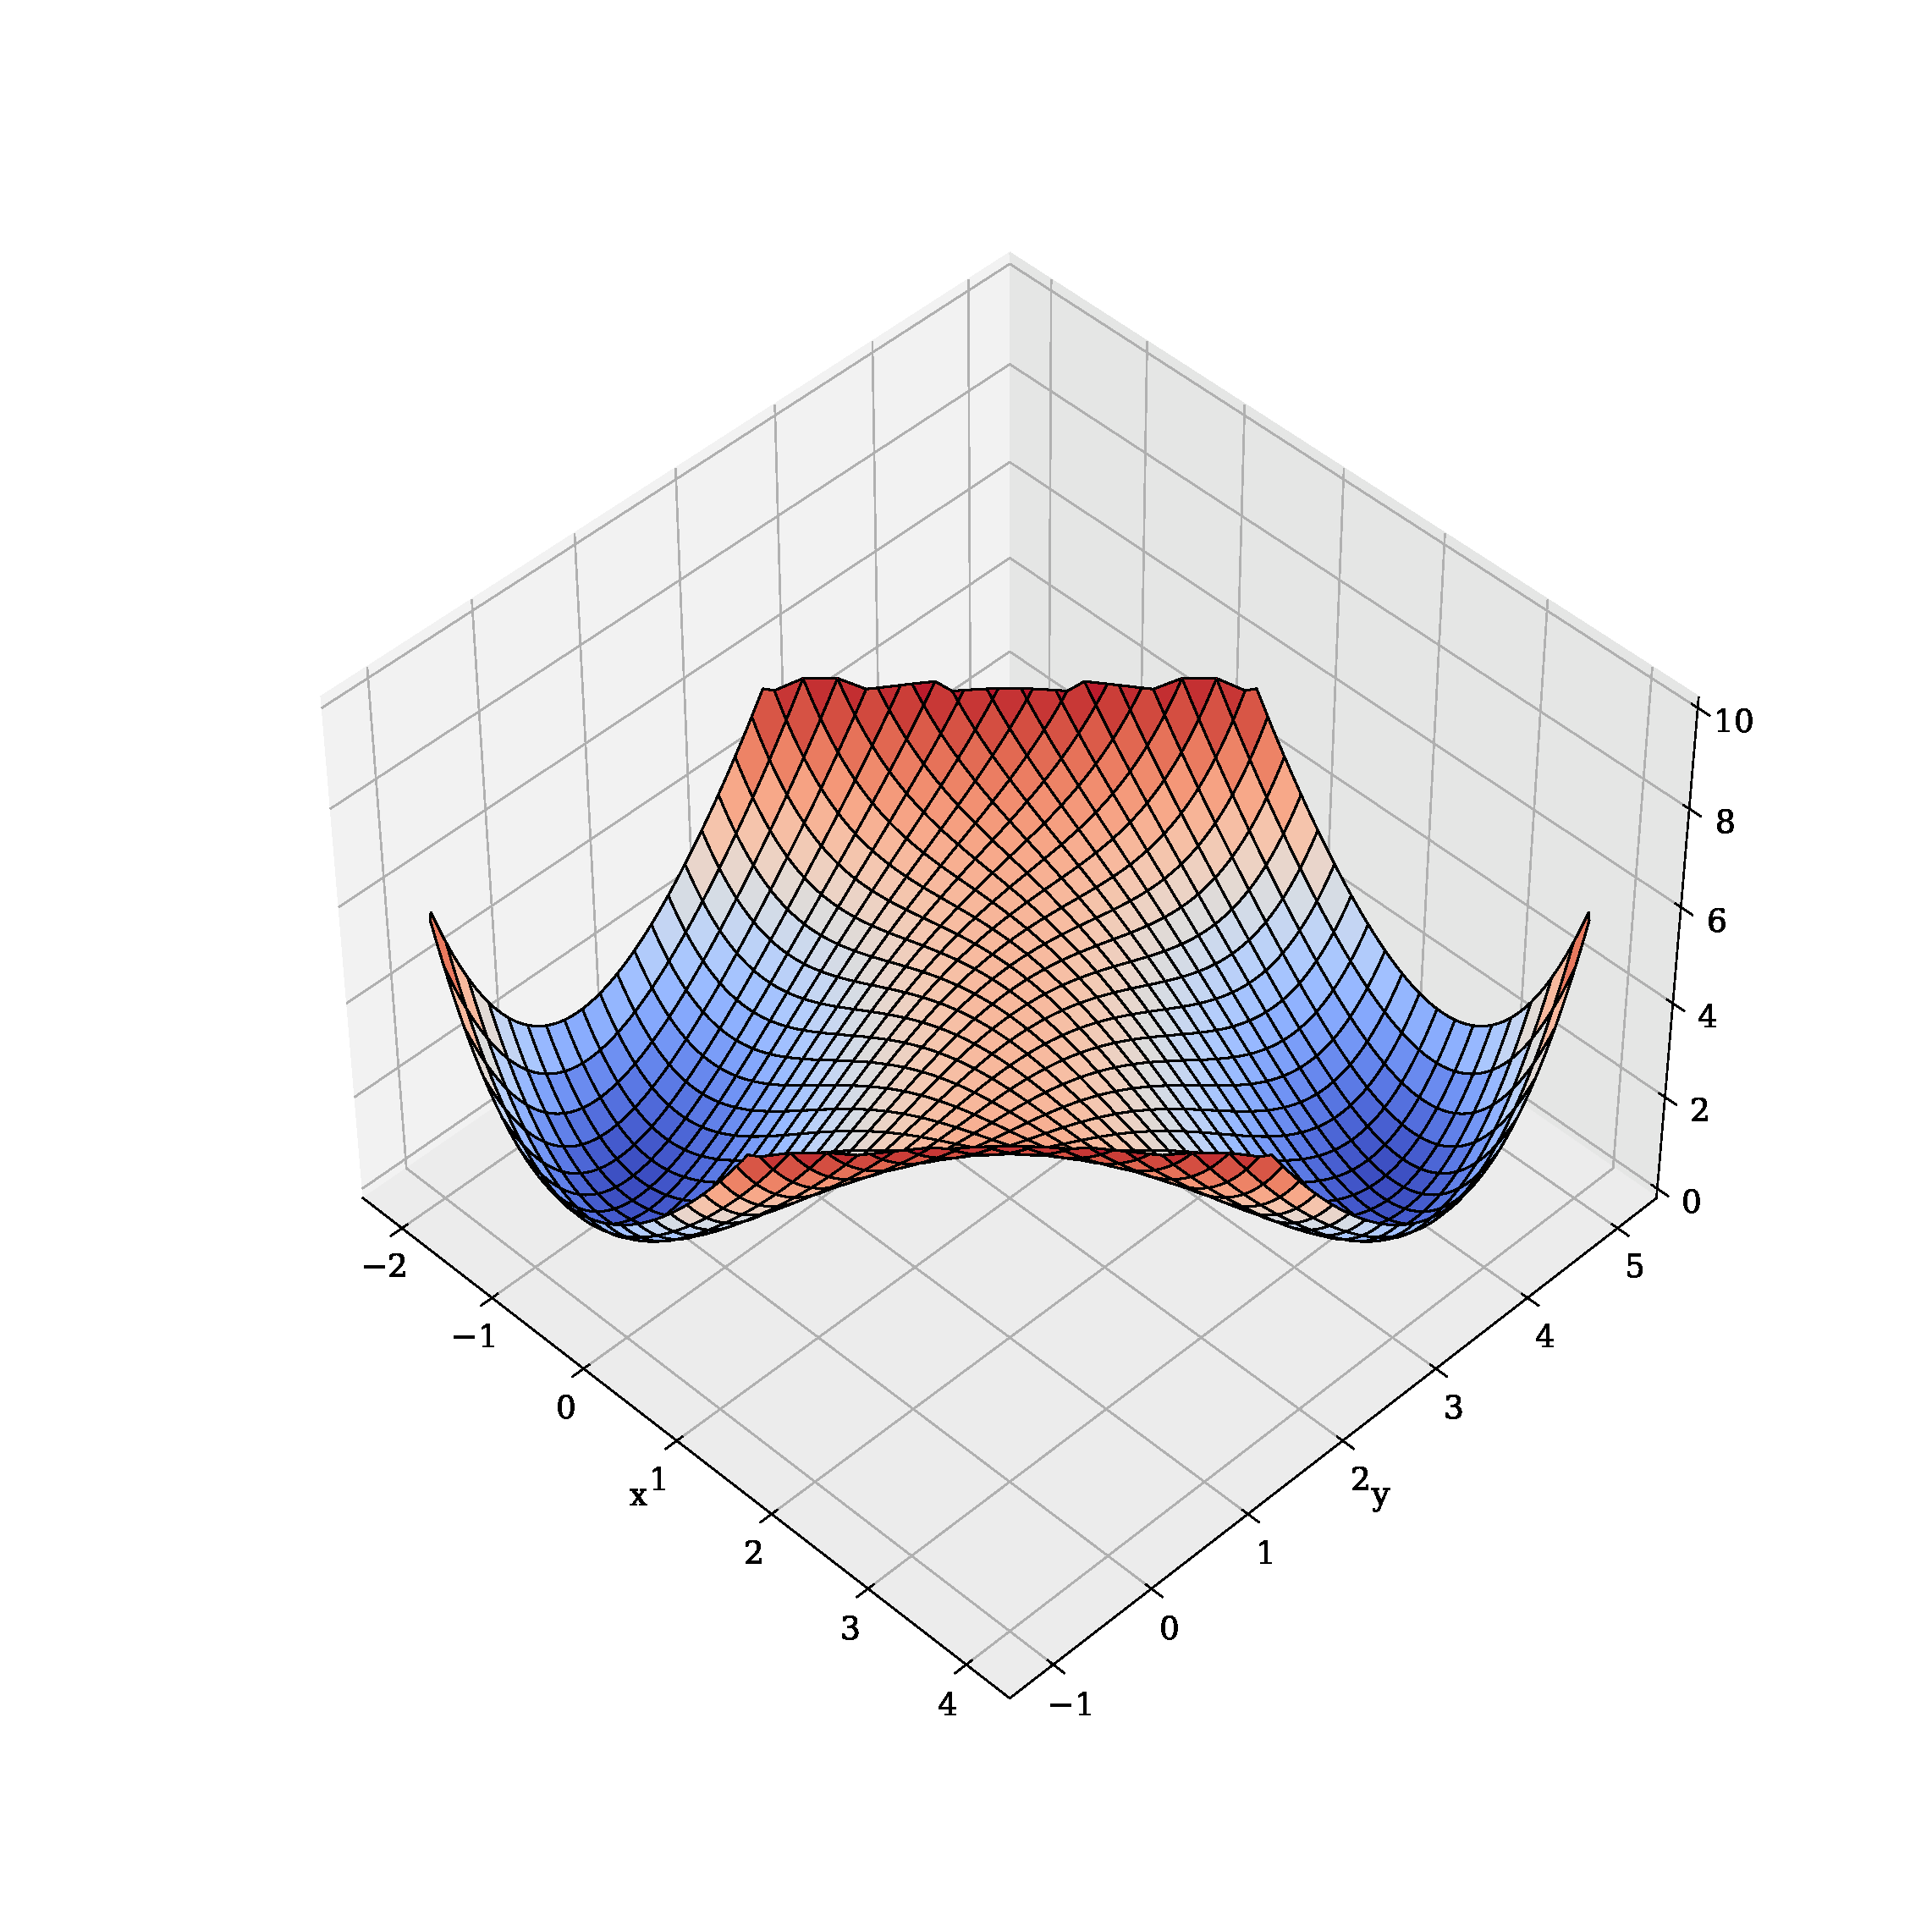
\includegraphics[width=0.8\textwidth]{NonConvex.eps}
		\label{fig:fig5}
	\end{center}
	\caption{Function $||\hat{\mathbf{\Sigma}}_{t+1} - \bar{\mathbf{\Sigma}}_{t+1}||_2^2$ for following series: $(1, 3)$ and $(2, 4)$. Minumums: (3; 4) is desired and (-1; 0) is alternative.}
\end{figure}


The problem with this method is the computational cost of non-convex optimisation methods. As an alternative, we propose the following method using only singular matrix decomposition.

{\textbf{Theorem 3. (Efficient method for obtaining a pair of possible answers.)} \textit{ The minimum of the function $||\hat{\mathbf{\Sigma}}_{t+1} - \bar{\mathbf{\Sigma}}_{t+1}||_2^2$ is reached on \[\pm\sqrt{\lambda_1} \mathbf{u}_1 + \boldsymbol{\mu}_t,\] where $\lambda_1$ is the first singular value, $\mathbf{u}_1$ is the first left singular vector of matrix $\mathbf{A}=\left(\hat{\mathbf{\Sigma}}_{t+1} - \frac{t}{t+1} \cdot \mathbf{\Sigma}_t \right) \cdot \frac{(t+1)^2}{t}$}

\textbf{Proof.} The notation $\mathbf{x}_i$ is used below to denote the \textit{multidimensional} value of the time series at time $i$. The proof expresses $\mathbf{\Sigma}_{t+1}$ through $\mathbf{\Sigma}_t$. After that, the operator norm and rank property of the matrix is used. All expressions below are true for arbitrary $\boldsymbol{\mu}_T$ and $\mathbf{\Sigma}_T$ constructed by the definition above.
\begin{enumerate}
	\item Express $\boldsymbol{\mu}$ through the values of the time series: \[\boldsymbol{\mu}_t = \frac{1}{t} \sum_{i=1}^{t} \mathbf{x}_i \Rightarrow \sum_{i=1}^{t} \mathbf{x}_i = t \boldsymbol{\mu}_t.\]
	\item Similarly, express $\mathbf{\Sigma_t}$ through the values of the series:
		\begin{gather*}
		\mathbf{\Sigma}_t = \frac{1}{t} \sum_{i=1}^{t} (\mathbf{x}_i-\boldsymbol{\mu}_t)(\mathbf{x}_i-\boldsymbol{\mu}_t)^\intercal;\\
		\mathbf{\Sigma}_t = \frac{1}{t} \sum_{i=1}^{t} \mathbf{x}_i \mathbf{x}_i^\intercal - \frac{1}{t} \left( \sum_{i=1}^{t} \mathbf{x}_i\right) \boldsymbol{\mu}_t^\intercal - \boldsymbol{\mu}_t \frac{1}{t} \left( \sum_{i=1}^{t} \mathbf{x}_i^\intercal\right) + \boldsymbol{\mu}_t \boldsymbol{\mu}_t^\intercal = \frac{1}{t} \sum_{i=1}^{t} \mathbf{x}_i \mathbf{x}_i^\intercal - \boldsymbol{\mu}_t \boldsymbol{\mu}_t^\intercal \Rightarrow\\
		\sum_{i=1}^{t} \mathbf{x}_i \mathbf{x}_i^\intercal = t \mathbf{\Sigma}_t + t \boldsymbol{\mu}_t \boldsymbol{\mu}_t^\intercal.
		\end{gather*}
	\item Express $\mathbf{\Sigma_{t+1}}$ through $\mathbf{\Sigma_t}$ using the previous expressions:
	\begin{gather*}
		\mathbf{\Sigma}_{t+1} = \frac{1}{t+1} \left(\sum_{i=1}^{t} \mathbf{x}_i \mathbf{x}_i^\intercal + \mathbf{x}_{t+1} \mathbf{x}_{t+1}^\intercal \right) - \boldsymbol{\mu}_{t+1} \boldsymbol{\mu}_{t+1}^\intercal = \\
		= \frac{t}{t+1}\mathbf{\Sigma}_t + \frac{t}{t+1}\boldsymbol{\mu}_{t} \boldsymbol{\mu}_{t}^\intercal + \frac{1}{t+1} \mathbf{x}_{t+1} \mathbf{x}_{t+1}^\intercal - \frac{1}{(t+1)^2} (t \boldsymbol{\mu}_t + \mathbf{x}_{t+1})(t \boldsymbol{\mu}_t + \mathbf{x}_{t+1})^\intercal =\\
		= \frac{t}{t+1}\mathbf{\Sigma}_t + \frac{t}{t+1}\boldsymbol{\mu}_{t} \boldsymbol{\mu}_{t}^\intercal + \frac{t}{(t+1)^2} \mathbf{x}_{t+1} \mathbf{x}_{t+1}^\intercal - \frac{t^2}{(t+1)^2}\boldsymbol{\mu}_{t} \boldsymbol{\mu}_{t}^\intercal - \frac{t}{(t+1)^2}\boldsymbol{\mu}_{t} \mathbf{x}_{t+1}^\intercal - \frac{t}{(t+1)^2}\mathbf{x}_{t+1} \boldsymbol{\mu}_{t}^\intercal =\\
		= \frac{t}{t+1}\mathbf{\Sigma}_t + \frac{t}{t+1}\boldsymbol{\mu}_{t} \boldsymbol{\mu}_{t}^\intercal - \frac{t}{(t+1)^2} \left( -\mathbf{x}_{t+1} \mathbf{x}_{t+1}^\intercal + t\boldsymbol{\mu}_{t} \boldsymbol{\mu}_{t}^\intercal + \boldsymbol{\mu}_{t} \mathbf{x}_{t+1}^\intercal + \mathbf{x}_{t+1} \boldsymbol{\mu}_{t}^\intercal \right) =\\
		= \frac{t}{t+1}\mathbf{\Sigma}_t + \frac{t}{t+1}\boldsymbol{\mu}_{t} \boldsymbol{\mu}_{t}^\intercal - \frac{t}{(t+1)^2} \left( -(\mathbf{x}_{t+1}-\boldsymbol{\mu}_t)(\mathbf{x}_{t+1}-\boldsymbol{\mu}_t)^\intercal + (t+1)\boldsymbol{\mu}_{t} \boldsymbol{\mu}_{t}^\intercal \right) =\\
		= \frac{t}{t+1}\mathbf{\Sigma}_t + \frac{t}{t+1}\boldsymbol{\mu}_{t} \boldsymbol{\mu}_{t}^\intercal - \frac{t(t+1)}{(t+1)^2}\boldsymbol{\mu}_{t} \boldsymbol{\mu}_{t}^\intercal + \frac{t}{(t+1)^2}(\mathbf{x}_{t+1}-\boldsymbol{\mu}_t)(\mathbf{x}_{t+1}-\boldsymbol{\mu}_t)^\intercal =\\
		= \frac{t}{t+1}\mathbf{\Sigma}_t + \frac{t}{(t+1)^2}(\mathbf{x}_{t+1}-\boldsymbol{\mu}_t)(\mathbf{x}_{t+1}-\boldsymbol{\mu}_t)^\intercal.
	\end{gather*}
	This equality expresses $\mathbf{\Sigma}_{t+1}$ through $\mathbf{\Sigma}_t$. For further proof it is useful to derive the following equality for our problem: \[(\bar{\mathbf{x}}_{t+1}-\boldsymbol{\mu}_t)(\bar{\mathbf{x}}_{t+1}-\boldsymbol{\mu}_t)^\intercal = \left(\bar{\mathbf{\Sigma}}_{t+1} - \frac{t}{t+1} \cdot \mathbf{\Sigma}_t \right) \cdot \frac{(t+1)^2}{t}.\]
	
	\item We solve the problem of finding the minimum of the function $||\hat{\mathbf{\Sigma}}_{t+1} - \bar{\mathbf{\Sigma}}_{t+1}||_2^2$. In our case, this is analogous to the equality of this function to zero. Let us write the expression under the norm:
	\begin{gather*}
		\hat{\mathbf{\Sigma}}_{t+1} - \bar{\mathbf{\Sigma}}_{t+1} = \frac{t}{t+1}\mathbf{\Sigma}_t + \frac{t}{(t+1)^2}(\hat{\mathbf{x}}_{t+1}-\boldsymbol{\mu}_t)(\hat{\mathbf{x}}_{t+1}-\boldsymbol{\mu}_t)^\intercal - \frac{t}{t+1}\mathbf{\Sigma}_t + \frac{t}{(t+1)^2}(\bar{\mathbf{x}}_{t+1}-\boldsymbol{\mu}_t)(\bar{\mathbf{x}}_{t+1}-\boldsymbol{\mu}_t)^\intercal =\\
		=\frac{t}{(t+1)^2}(\hat{\mathbf{x}}_{t+1}-\boldsymbol{\mu}_t)(\hat{\mathbf{x}}_{t+1}-\boldsymbol{\mu}_t)^\intercal -\frac{t}{(t+1)^2}(\bar{\mathbf{x}}_{t+1}-\boldsymbol{\mu}_t)(\bar{\mathbf{x}}_{t+1}-\boldsymbol{\mu}_t)^\intercal.
 	\end{gather*}
 	Then, the problem above is equivalent to finding the minimum of the function \[||(\hat{\mathbf{x}}_{t+1}-\boldsymbol{\mu}_t)(\hat{\mathbf{x}}_{t+1}-\boldsymbol{\mu}_t)^\intercal-(\bar{\mathbf{x}}_{t+1}-\boldsymbol{\mu}_t)(\bar{\mathbf{x}}_{t+1}-\boldsymbol{\mu}_t)^\intercal||_2^2.\]
 	Denote \[\mathbf{A} = (\bar{\mathbf{x}}_{t+1}-\boldsymbol{\mu}_t)(\bar{\mathbf{x}}_{t+1}-\boldsymbol{\mu}_t)^\intercal = \left(\bar{\mathbf{\Sigma}}_{t+1} - \frac{t}{t+1} \cdot \mathbf{\Sigma}_t \right) \cdot \frac{(t+1)^2}{t}.\]
 	The rank of the matrix ($\hat{\mathbf{x}}_{t+1}-\boldsymbol{\mu}_t)(\hat{\mathbf{x}}_{t+1}-\boldsymbol{\mu}_t)^\intercal$ is 1, and since the desired minimum is 0, it turns out that the rank of the matrix $\mathbf{A}$ is also 1.
 	
 	\item From the previous paragraph, the matrix $\mathbf{A}$ has rank 1. Let us write the singular value decomposition. \[
 		\mathbf{A} = \sum_{i=1}^{1} \lambda_i \mathbf{u}_i \mathbf{v}_i^\intercal = \lambda_1 \mathbf{u}_1 \mathbf{v}_1^\intercal.
 	\]
 	On the other hand, $\mathbf{A} = (\bar{\mathbf{x}}_{t+1}-\boldsymbol{\mu}_t)(\bar{\mathbf{x}}_{t+1}-\boldsymbol{\mu}_t)^\intercal$. Then, \[
 	\bar{\mathbf{x}}_{t+1}-\boldsymbol{\mu}_t = \pm\sqrt{\lambda_1} \mathbf{u}_1 \Leftrightarrow\\
 	\bar{\mathbf{x}}_{t+1} = \pm\sqrt{\lambda_1} \mathbf{u}_1 + \boldsymbol{\mu}_t.
 	\]
 	The sign $\pm$ comes from the fact that in the case of a symmetric matrix, there are two singular value decompositions: $\mathbf{A}=\mathbf{U}\mathbf{\Sigma} \mathbf{V}^\intercal=(-\mathbf{U})\mathbf{\Sigma} (-\mathbf{V})^\intercal$.
 	$$ \blacksquare $$
\end{enumerate}

This theorem allows us to find both minimums of a function much faster than with standard non-convex optimisation methods \cite{mikhalevich2024methodsnonconvexoptimization}.

\section{Algorithm for recovering time series values in case of accurate prediction of the matrix}

Theorems 2 and 3 show that using a single pairwise correlation matrix and information about the first $t$ moments of time allows us to obtain a \textit{pair} of possible values after recovery. In this section, we propose a method to select the true value from the obtained \textit{pair} $\mathbf{\Sigma}_{t+1}$ \textit{predicted accurately}.

The algorithm described below is based on the use of \textit{two} predicted matrices corresponding to different intervals of time. Two different values $T, T^\prime$ are chosen. Two matrices are predicted:

First $\mathbf{\Sigma}_{t+1}^1$ pairwise correlation matrix for the multivariate time series $\mathbf{x}$ at time moments from $t-T+2$ to $t+1$ (in total $T$ values).

Second $\mathbf{\Sigma}_{t+1}^2$ pairwise correlation matrix for the multivariate time series $\mathbf{x}$ at time moments from $t-T‘+2$ to $t+1$ (in total $T^\prime$ values).

Hence, when we reconstruct answers from these matrices, we obtain two pairs of answers, each of which is a candidate for the true answer. At the same time, a true answer exists in each of the pairs. It is suggested to take the answer from the intersection. We does not consider the case when the intersection size is 2, since the probability of this situation is 0 when using continuous values.

Algorithm scheme:

\begin{enumerate}
	\item Take $T$ and $T^\prime: T \neq T'$.
	\item For $T$ and $T^\prime$ perform the above algorithm and obtain the answer sets: \[ [\hat{\mathbf{x}}_{t+1}^1, \hat{\mathbf{x}'}_{t+1}^1], [\hat{\mathbf{x}}_{t+1}^2, \hat{\mathbf{x}'}_{t+1}^2].\]
	\item Find the answer that lies in the intersection.
	In real data, the probability of matching sets of answers is 0, just as it is in synthetic data with random noise added.
\end{enumerate}


\begin{figure}[H]
	\centering
	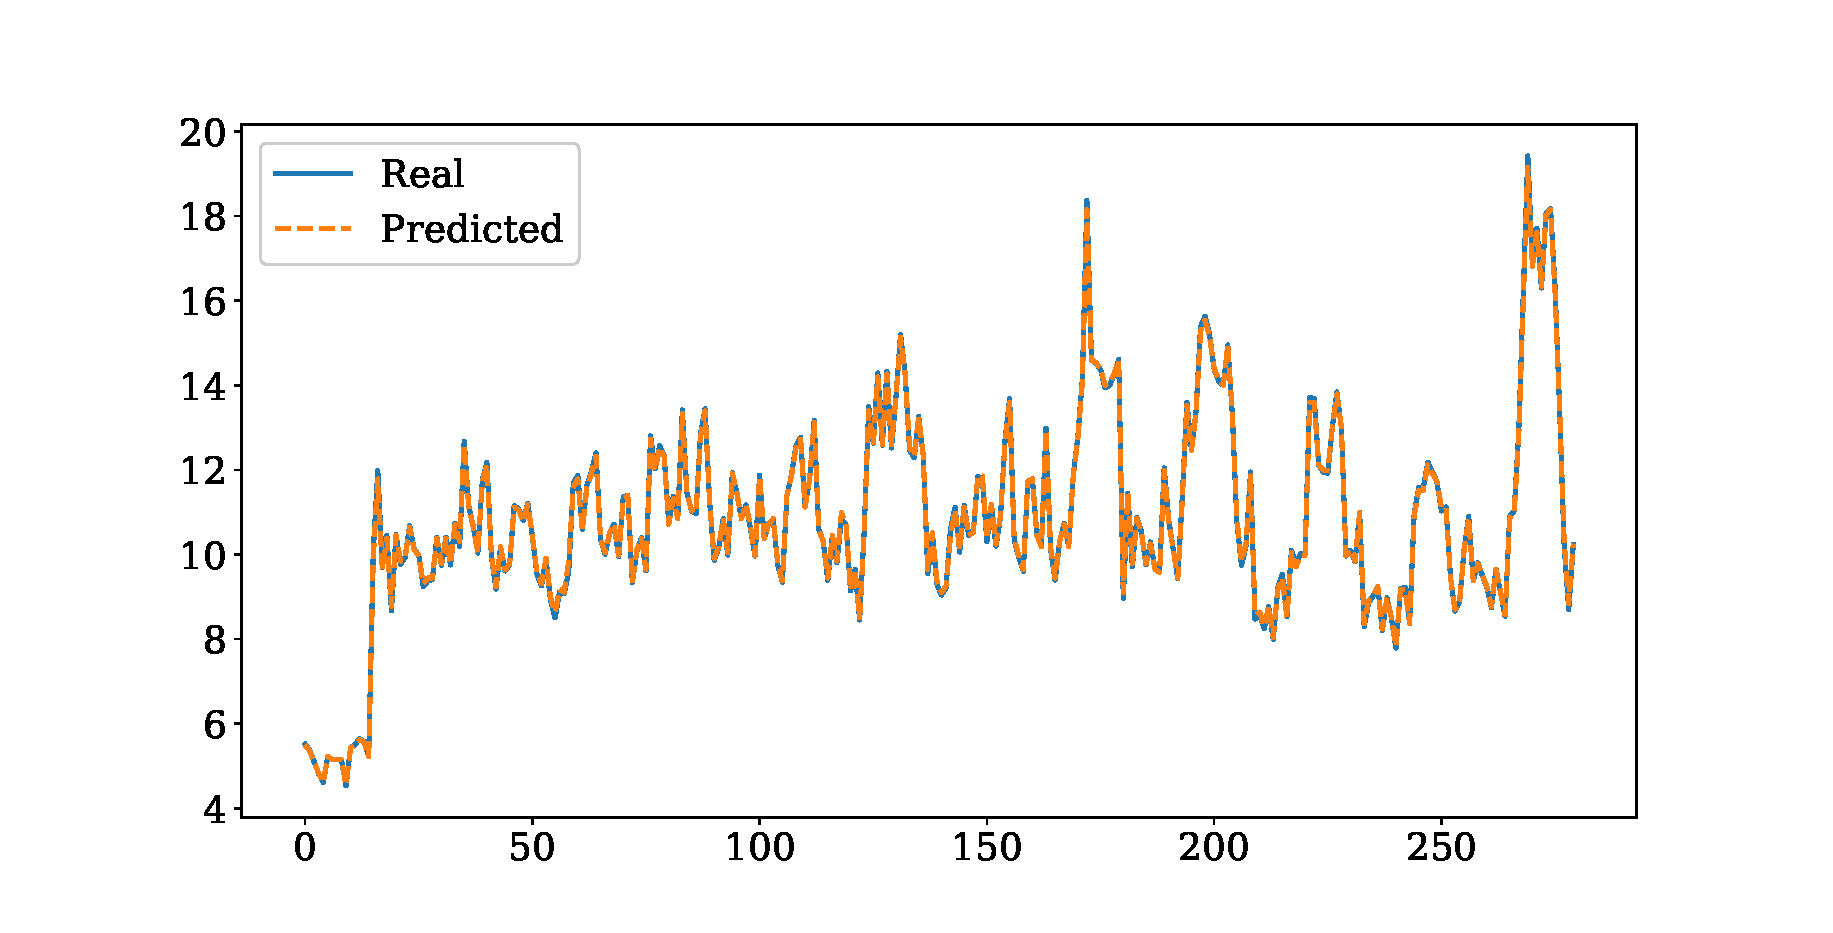
\includegraphics[width=\textwidth]{IdealRecovery.eps}
	\caption{Prediction recovery in case of accurate prediction of correlation matrix $\mathbf{\Sigma}$. $T=20$, $T^\prime=10$}
	\label{fig:fig3}
\end{figure}

\section{Algorithm for recovering time series values in case of inaccurate matrix prediction}

The problem with the above algorithm is that if the prediction is inaccurate, there may be no intersection. This happens because the error in each of the predicted matrices is different. For this, the following algorithm is proposed to amortise the error:

Instead of two values of $T$ and $T^\prime$, $K$ values are taken.
Next, each matrix is reduced to the nearest positive semi-definite matrix.
Then we get $K$ sets of answers:
\begin{gather*}
	[\hat{\mathbf{x}}_{t+1}^1, \hat{\mathbf{x}}^{\prime 1}_{t+1}],\\
	[\hat{\mathbf{x}}_{t+1}^2, \hat{\mathbf{x}}^{\prime 2}_{t+1}],\\
	\vdots \\
	[\hat{\mathbf{x}}_{t+1}^K, \hat{\mathbf{x}}^{\prime K}_{t+1}].
\end{gather*}
Then we propose to search through $2^K$ sets of answers and choose the set in which the diameter is minimal. The diameter of set is calculated as maximum Euclidean distance between two different points in set. It is a \textit{necessary} condition for the actual answer. In other words, the one that is the intersection of all pairs of answers. In the case of an accurate prediction, the diameter of such a set will always be zero.

The asymptotic complexity of this recovery will be $O(2^K \times K \times N)$ $+$ the complexity of the minimum search algorithm used.
\begin{figure}[H]
	\centering
	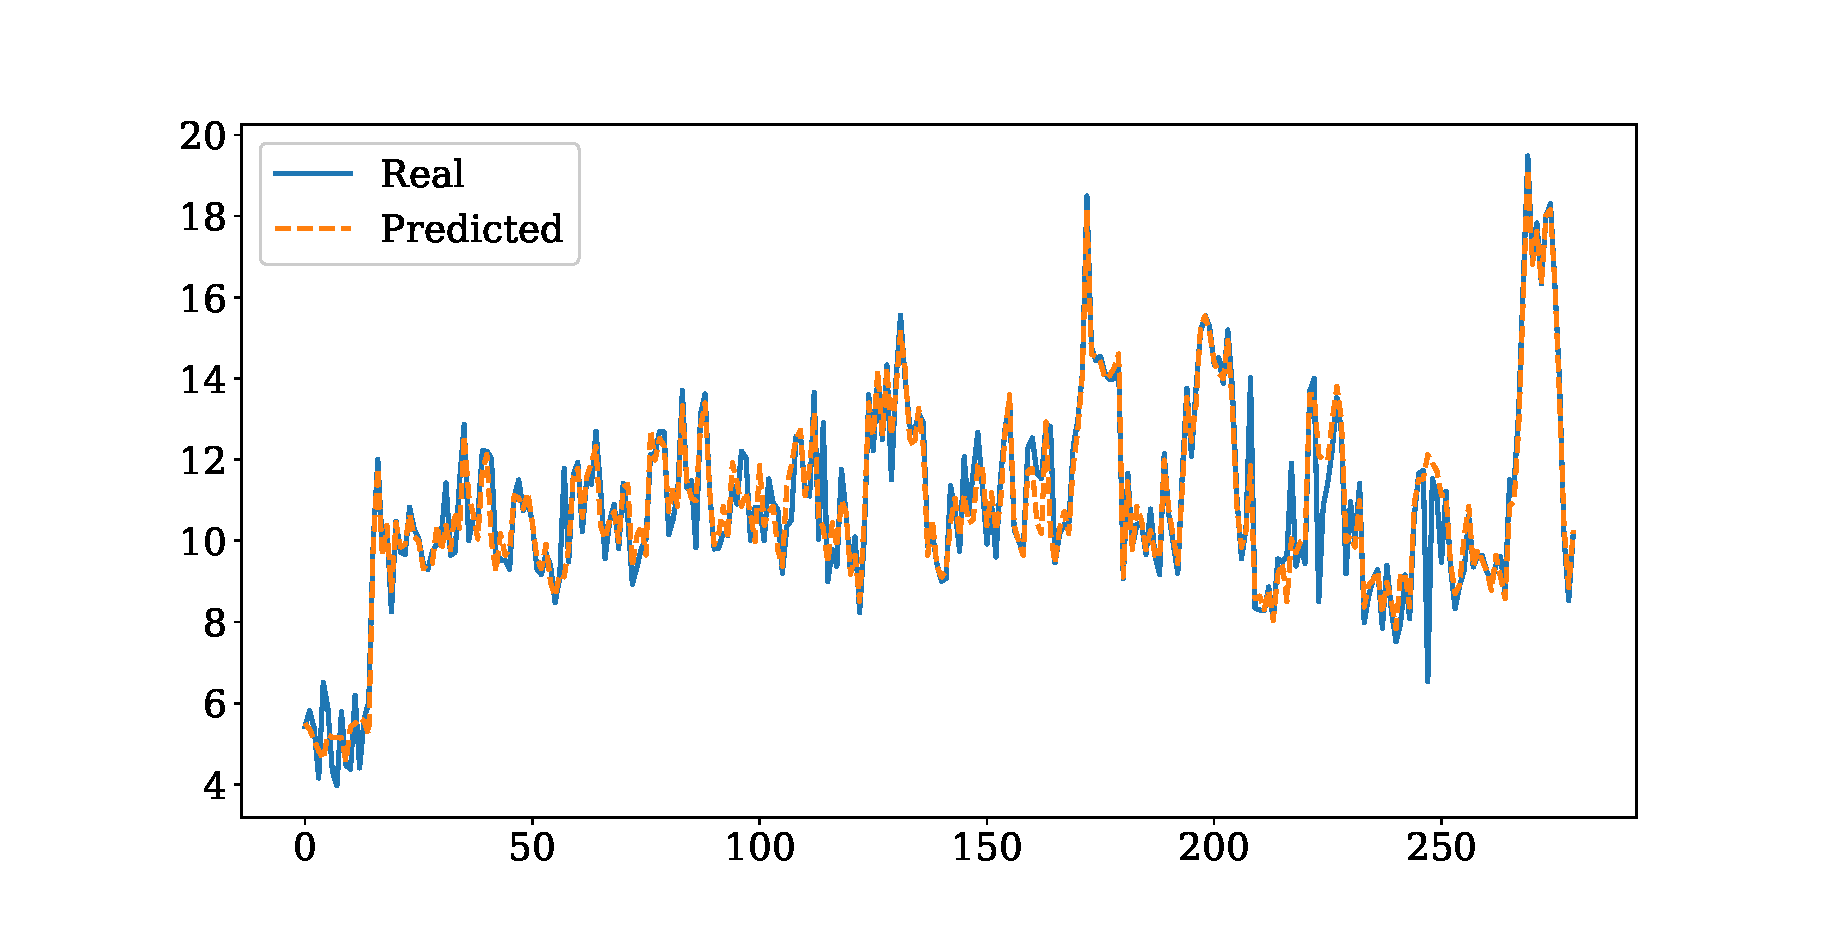
\includegraphics[width=\textwidth]{NonIdealRecovery.eps}
	\caption{Prediction recovery in case of inaccurate correlation matrix $\mathbf{\Sigma}$ prediction. In addition to the prediction error caused by noise in the correlation matrix a new type of error is added. When selecting a set, it is possible that the diameter is minimised not at the right set, as this is only a necessary condition, but not a sufficient one.}
	\label{fig:fig4}
\end{figure}

\section{Experiment}

In this section we test the algorithm when the pairwise correlation matrix prediction from the previous section is inaccurate. Experiments are performed on synthetic data as well as on Electricity Transformer Temperature \cite{zhou2021informer} data. Different values of $K$ are tested, as well as different added noise to the true matrix values.

\paragraph{Synthetic data.}\

The table below shows the error values after recovery under different conditions. Generated data consisting of a combination of noisy sines and cosines are used.

\begin{table}[!h]
\def\arraystretch{2.3}
\begin{center}
\caption{Loss on synthetic data}
\begin{tabular}{|l||l||*{3}{c|}}\hline
	\backslashbox{Noise}{Parameters}
	&\makebox[3em]{Metric}&\makebox[3em]{$K=2$}&\makebox[3em]{$K=4$}&\makebox[3em]{$K=10$}\\\hline
	$\mathcal{N}(0, 0.01)$&\makecell{ MAE: \\ MSE: } &\makecell{ 0.070 \\ 0.010 }&\makecell{ 0.052 \\ 0.005 }&\makecell{ 0.040 \\ 0.002 }\\\hline
	$\mathcal{N}(0, 0.05)$&\makecell{ MAE: \\ MSE: } &\makecell{ 0.316 \\ 0.295 }&\makecell{ 0.176 \\ 0.060 }&\makecell{ 0.116 \\ 0.025 }\\\hline
	$\mathcal{N}(0, 0.1)$& \makecell{ MAE: \\ MSE: } &\makecell{ 0.530 \\ 0.635 }&\makecell{ 0.398 \\ 0.348 }&\makecell{ 0.230 \\ 0.111 }\\\hline
\end{tabular}
\end{center}
\end{table}


\begin{figure}[H]
	\centering
	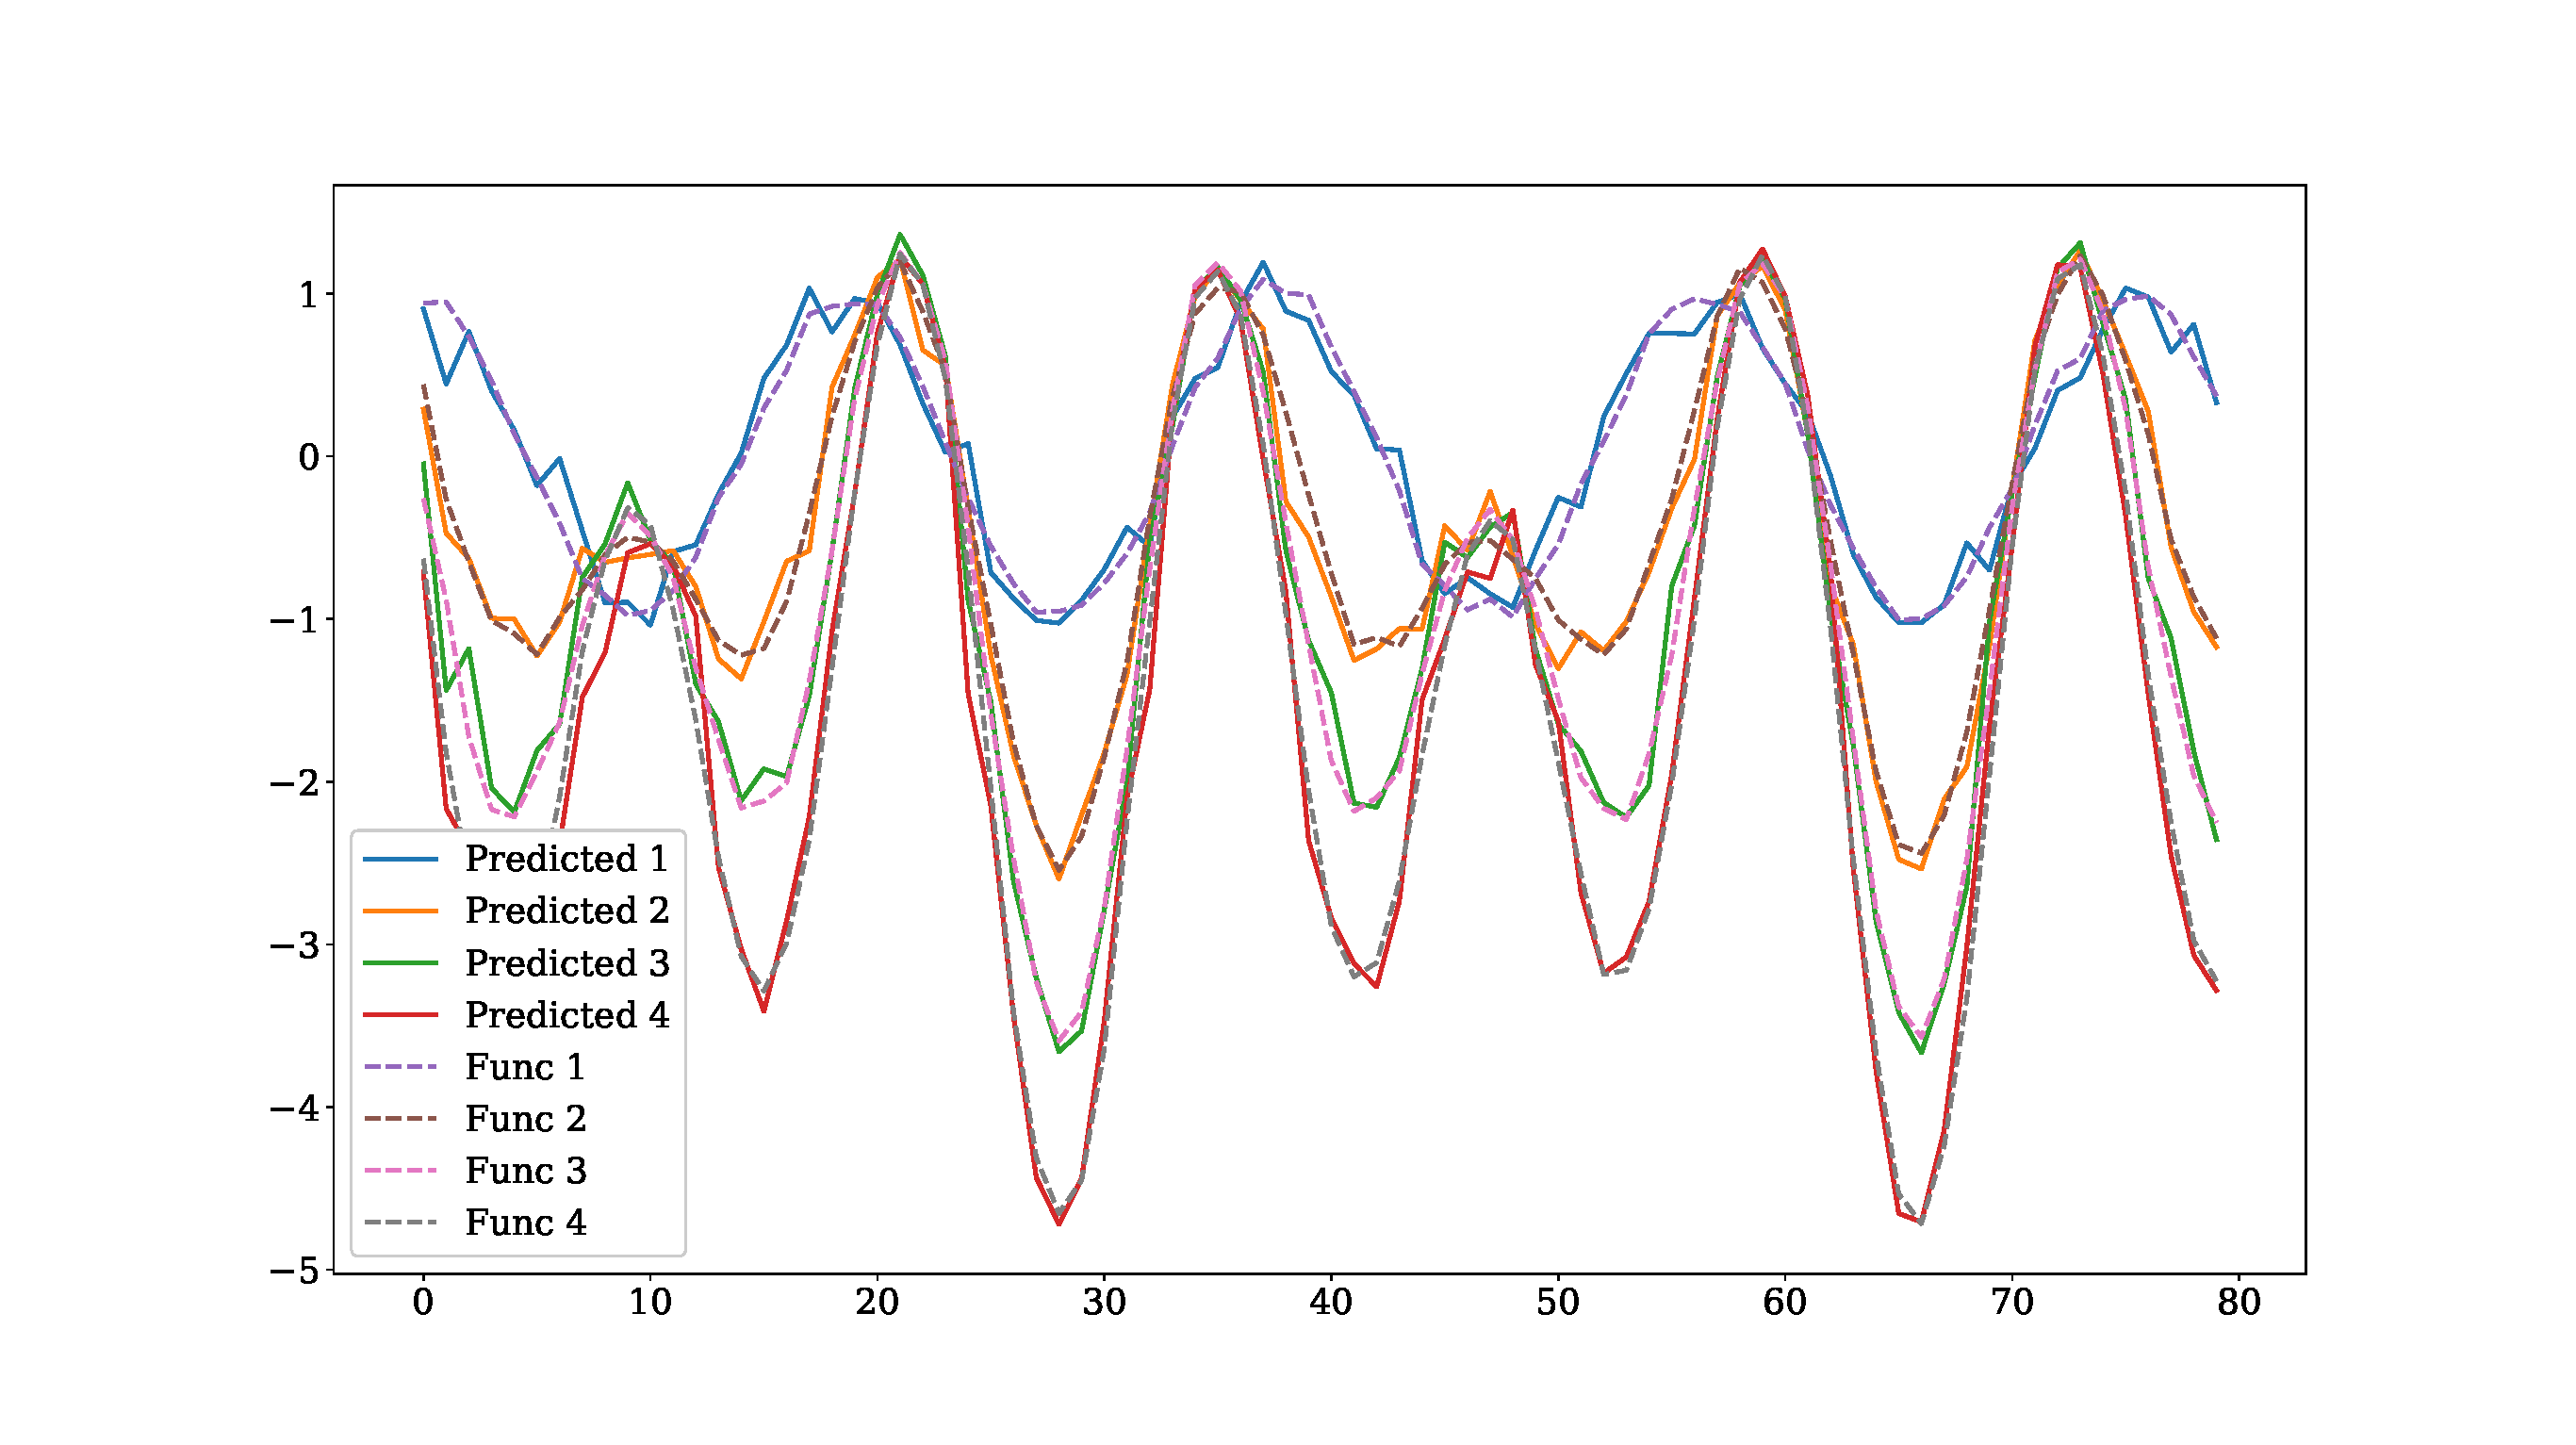
\includegraphics[width=\textwidth]{synthetic_time_series_K10N005.eps}
	\caption{Synthetic data recovery plot at $K=10$, Additional noise $\mathcal{N}(0, 0.05)$. \textbf{MAE: 0.116, MSE: 0.025}}
	\label{fig:fig6}
\end{figure}

\paragraph{Electricity Transformer Temperature}\

The following is a similar table for the Electricity Transformer Temperature dataset.

\begin{figure}[H]
	\centering
	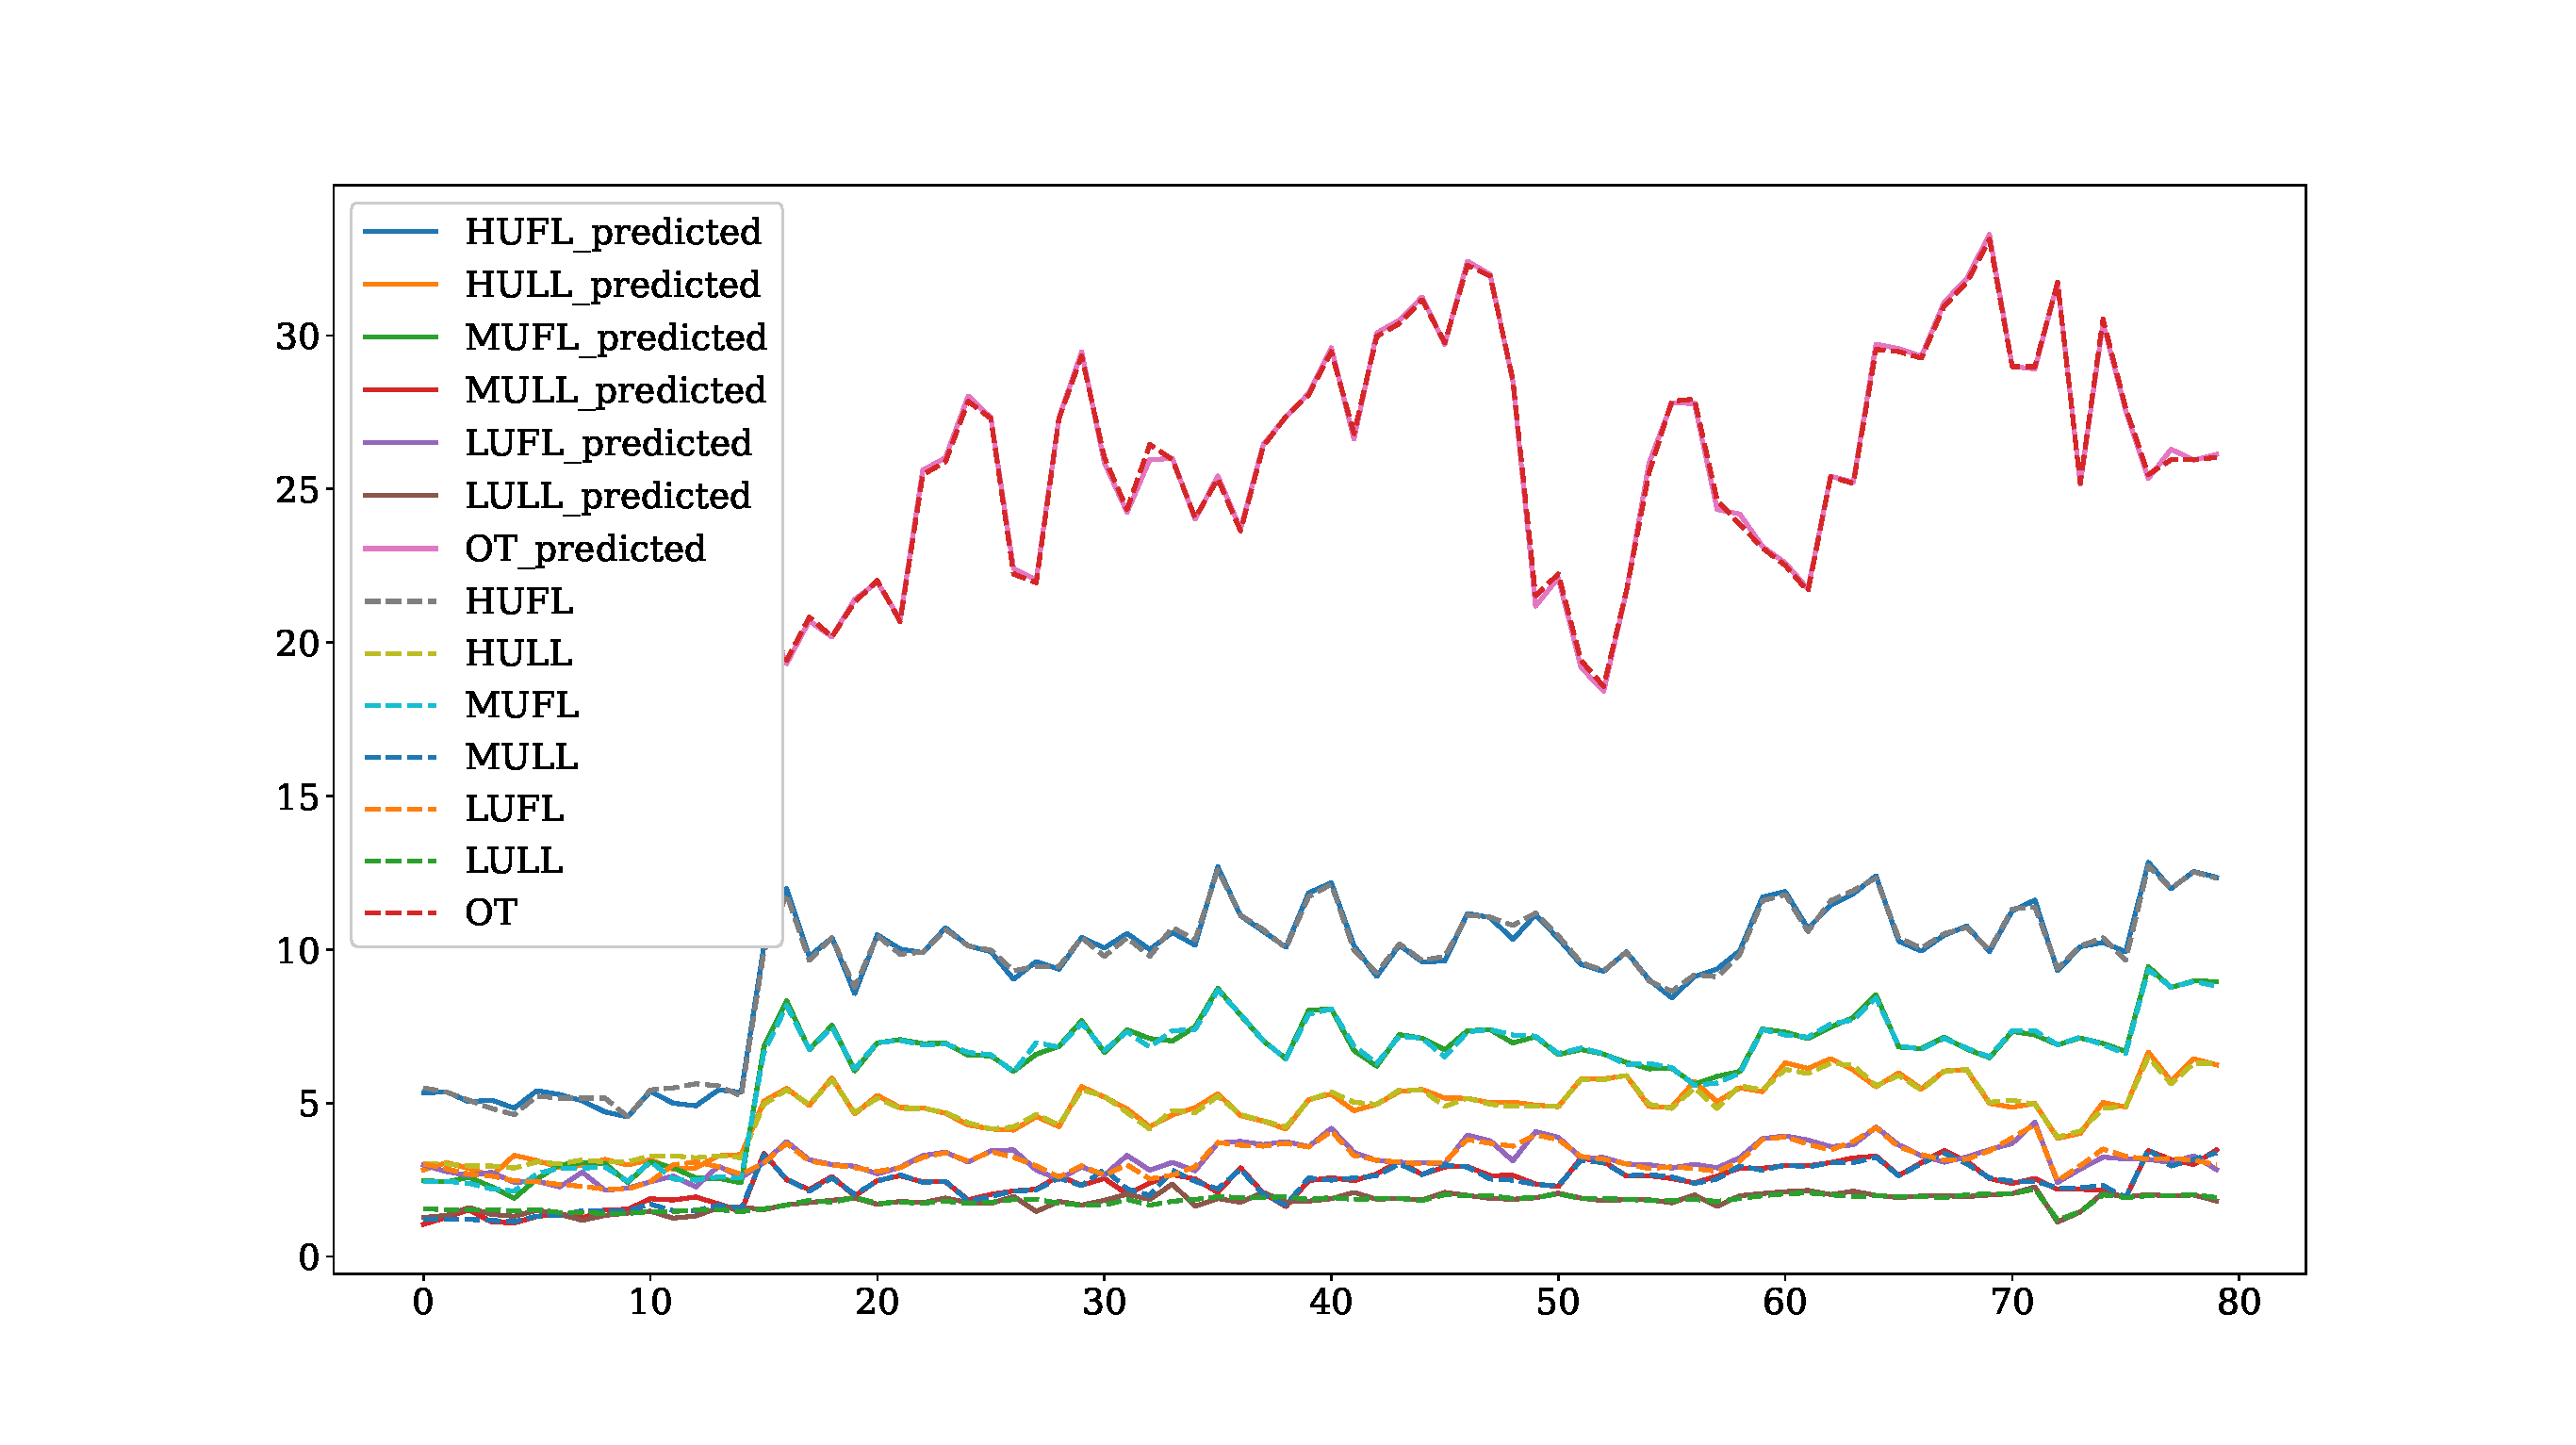
\includegraphics[width=\textwidth]{ETT_time_series_K10N005.eps}
	\caption{ETTh1 data recovery plot at $K=10$, Additional Noise $\mathcal{N}(0, 0.05)$. \textbf{MAE: 0.096, MSE: 0.019}}
	\label{fig:fig7}
\end{figure}

\begin{table}[!h]
\def\arraystretch{2.3}
\begin{center}
\caption{Loss on ETTh1 data}
\begin{tabular}{|l||l||*{3}{c|}}\hline
	\backslashbox{Noise}{Parameters}
	&\makebox[3em]{Metric}&\makebox[3em]{$K=2$}&\makebox[3em]{$K=4$}&\makebox[3em]{$K=10$}\\\hline
	$\mathcal{N}(0, 0.01)$&\makecell{ MAE: \\ MSE: } &\makecell{ 0.071 \\ 0.030 }&\makecell{ 0.047 \\ 0.004 }&\makecell{ 0.038 \\ 0.003 }\\\hline
	$\mathcal{N}(0, 0.05)$&\makecell{ MAE: \\ MSE: } &\makecell{ 0.240 \\ 0.198 }&\makecell{ 0.153 \\ 0.053 }&\makecell{ 0.096 \\ 0.019 }\\\hline
	$\mathcal{N}(0, 0.1)$& \makecell{ MAE: \\ MSE: } &\makecell{ 0.466 \\ 0.719 }&\makecell{ 0.306 \\ 0.281 }&\makecell{ 0.217 \\ 0.148 }\\\hline
\end{tabular}
\end{center}
\end{table}


In all cases, using more different values of $T$ predictably gave the highest accuracy. However, for $K > 15$ the algorithm becomes too computationally complex due to the exponential dependence on $K$.

\section{Conclusion}
The paper investigates an approach to time series forecasting using a pairwise correlation matrix between series. It is shown that the use of only one matrix leads to the existence of a pair of possible answers~--- the values of the series at the next moment of time. An explicit formula for computing one answer through the other is derived, which allows the problem to be solved using nonconvex optimisation. Moreover, an explicit form of the pair of answers via the singular value decomposition of the pairwise correlation matrix is derived. Two algorithms are proposed to identify the desired answer from a pair of possible answers. The first one relies on the exact prediction of the pairwise correlation matrix. The second one admits the presence of an error in the prediction, but it is more computationally demanding.

The future development of the study is to find a way to predict the pairwise correlation matrix with high accuracy. Using basic regression models give insufficiently accurate results. In such a prediction, errors are often made by incorrectly selecting the set of answers from Algorithm 2. 

Also, the side of development can be the estimation of the error radius when recovering the value of time series from the matrix of pair correlations. In addition, it makes sense to consider other functions of pairwise distance as a metric.

\bibliography{references}
\bibliographystyle{plain}


\end{document}